\chapter{Introducción específica} % Main chapter title

\label{Chapter2}

%----------------------------------------------------------------------------------------
%	SECTION 1
%----------------------------------------------------------------------------------------
En este capítulo se detallan los aspectos técnicos específicos que constituyen la base del trabajo. En primer lugar, se describen los protocolos de comunicación que se emplean y la función de cada uno de ellos en la transmisión de datos. Luego, se presentan los componentes de hardware que utiliza el prototipo. A continuación, se analizan las tecnologías de software que integran la solución, la herramienta de control de versiones adoptada para el desarrollo colaborativo y la gestión del código fuente.

\section{Protocolos y comunicación}
El diseño de un sistema de conteo de tránsito con comunicación bidireccional demanda la incorporación de protocolos que aseguren confiabilidad y eficiencia en el intercambio de datos. En este trabajo se integran tres tecnologías principales: 

\begin{itemize}
	\item RS-232: es un estándar de comunicación serial utilizado tradicionalmente en sistemas embebidos. Permite la transmisión de datos punto a punto entre el contador de tránsito y el microcontrolador ESP32-C3 \cite{esp32c3}. Su simplicidad lo hace adecuado para distancias cortas y ambientes donde la interferencia es controlada. Aunque se trata de un protocolo clásico, su adopción garantiza compatibilidad con dispositivos que aún dependen de interfaces seriales \cite{analogRS232},  \cite{tiRS232}.
	
	\item MQTT: este protocolo de mensajería ligera se emplea tanto para la transmisión de eventos de tránsito desde los dispositivos hacia el servidor central como para la recepción de comandos en sentido inverso. MQTT opera sobre TCP/IP \cite{comerTCPIP} y emplea un modelo de publicación/suscripción a través de un broker, lo que facilita la escalabilidad y la integración de múltiples dispositivos. Además, permite implementar mecanismos de calidad de servicio (QoS) que reducen la probabilidad de pérdida de datos en condiciones de conectividad inestable, lo que resulta crucial para el escenario de rutas nacionales \cite{mqttSpec}.
	
	\item API REST: constituye la interfaz de comunicación entre el backend y los clientes web. Su inclusión en el trabajo posibilita la consulta y el envío de información de manera estructurada, mediante operaciones estándar (GET, POST, PUT, DELETE). La API REST asegura la interoperabilidad con diferentes plataformas y brinda flexibilidad para desarrollar aplicaciones adicionales que utilicen los datos recolectados \cite{ibmRest}, \cite{microsoftApiDesign} .
		
\end{itemize}

La combinación de estos protocolos permite cubrir distintos niveles de la arquitectura: comunicación local (RS-232), comunicación de dispositivos con el servidor (MQTT) y comunicación entre el servidor y las aplicaciones de usuario (API REST). De esta forma, se garantiza un flujo de datos seguro, confiable y bidireccional.



%----------------------------------------------------------------------------------------

\section{Componentes de hardware utilizados}

El prototipo se implementa con un conjunto de componentes de hardware seleccionados por su disponibilidad, costo y adecuación al entorno de operación:

\begin{itemize}

\item  Contador de tránsito: dispositivo de campo encargado de detectar y acumular el paso de vehículos y generar tramas de datos que contienen información de conteo, clasificación y marcas temporales. Estos equipos permiten registrar de manera continua el flujo vehicular en rutas nacionales y constituyen la base del sistema de monitoreo. Si bien en el mercado existen distintos contadores comerciales que ofrecen funcionalidades similares, muchos de ellos presentan altos costos de adquisición, dependencia de plataformas propietarias o limitaciones de integración. En este proyecto se optó por utilizar un contador desarrollado por la Dirección Nacional de Vialidad, el cual ha sido probado en distintos corredores viales del país y cuenta con una interfaz de salida RS-232 \cite{tiRS232} con un adaptador MAX232 \cite{max232}. Esta elección responde a criterios de soberanía tecnológica, optimización de recursos ya disponibles y reducción de costos. Además, el contador no solo transmite información de eventos, sino que también admite la recepción de comandos externos a través del nodo, lo que habilita funcionalidades de diagnóstico, reconfiguración remota y confirmación de estado. De este forma, se garantiza la compatibilidad con la infraestructura existente y se potencia su integración dentro de una arquitectura moderna basada en protocolos abiertos.

En la Figura \ref{fig:foto_dtec} se observa el contador de tránsito. Este dispositivo constituye la base del sistema de detección de eventos. 




\item ESP32-C3: microcontrolador de bajo consumo que actúa como unidad de procesamiento y comunicación. Integra conectividad y capacidad de comunicación serial, lo que lo hace adecuado para la interacción con el contador y con el módulo GPRS \cite{esp32c3IDF}.

\item Módulo GPRS SIM800L: permite la conexión de los dispositivos a la red celular \cite{sim800l_datasheet} , asegurando la transmisión de datos al servidor central mediante MQTT. Se eligió por su bajo costo, disponibilidad en el mercado y facilidad de integración con el ESP32-C3.

\item Servidor central: responsable de recibir los datos transmitidos, almacenarlos en una base de datos y responder a las solicitudes de los usuarios.

\item PC con navegador web: constituye el medio de interacción del usuario final con el sistema, a través de la interfaz desarrollada.

\item Fuente de alimentación: fuente principal con batería interna recargable y recarga mediante panel solar, capaz de cubrir los picos de consumo del SIM800L. Incluye regulador de tensión y capacitores que estabilizan el voltaje y evitan reinicios.

\item Carcasa y gabinete: protección para el contador y el módulo de comunicación (ESP32-C3 y SIM800L) en un gabinete cerrado resistente a humedad, polvo y vibraciones, con disipación térmica y reducción de interferencias electromagnéticas.

\item Componentes adicionales: filtros (capacitores) para garantizar estabilidad y evitar reinicios inesperados.


\end{itemize}



\begin{figure}[htbp]
  \centering
  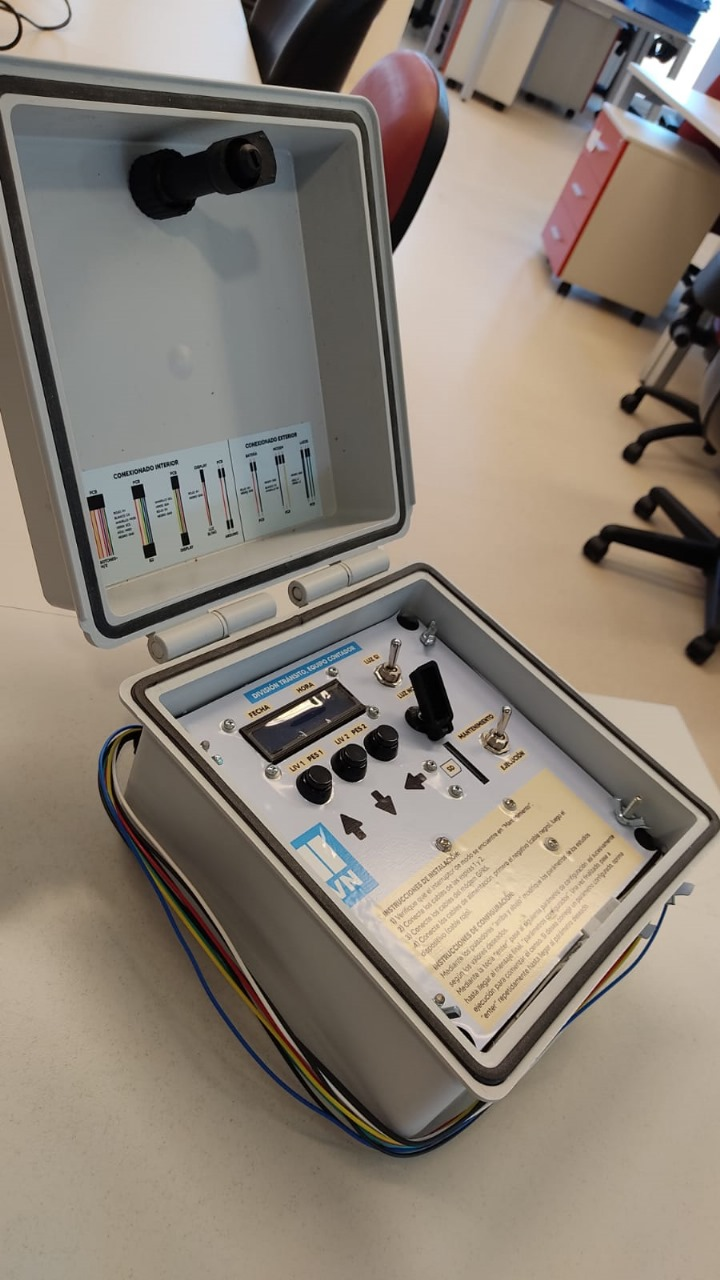
\includegraphics[width=0.4\linewidth]{./Figures/fotoDTEC.jpeg}
  \caption{Contador de tránsito DTEC \protect\footnotemark.}
  \label{fig:foto_dtec}
\end{figure}


\footnotetext{Imagen tomada de \url{http://transito.vialidad.gob.ar/}}
La integración de estos componentes asegura que el sistema pueda operar en condiciones reales y que cumpla con los requisitos.


\section{Tecnologías de software aplicadas}
El desarrollo del prototipo se sustenta en tecnologías de software abiertas y estandarizadas, seleccionadas por su solidez, disponibilidad y capacidad de integración.

\begin{itemize}

\item MQTT con Eclipse Mosquitto. 
La mensajería ligera y bidireccional se implementa mediante el protocolo MQTT, operando sobre el broker Eclipse Mosquitto \cite{mosquitto}. Este software es ampliamente utilizado en entornos de Internet de las Cosas (IoT).

\item API REST con Node.js  y Express. 
El backend se desarrolla en Node.js \cite{nodejs}, un entorno de ejecución orientado a aplicaciones de red no bloqueantes, y se estructura con Express \cite{expressjs}, un framework ligero que facilita la creación de servicios RESTful.

\item Base de datos relacional MySQL. 
La persistencia de los datos se implementa en MySQL \cite{mysql}, un sistema gestor de bases de datos relacionales ampliamente adoptado. En ella se almacenan de manera estructurada tanto los eventos de tránsito como los estados reportados por los equipos.

\item ORM con Sequelize.
Para abstraer la interacción con la base de datos y mantener independencia frente a cambios en la capa de persistencia, se utiliza Sequelize \cite{sequelize}, un ORM para Node.js que permite definir modelos y relaciones de manera declarativa.  

\item Sistema de logging con Winston.
La trazabilidad de eventos y errores se gestiona mediante Winston \cite{winston}, una librería de logging que soporta múltiples transportes y permite configurar niveles de severidad, formatos y timestamps.  

\item Middleware de registro HTTP con Morgan.
Para capturar y auditar el tráfico entrante al backend se emplea Morgan \cite{morgan}, un middleware especializado en logging de peticiones HTTP, complementando la funcionalidad de Winston.  

\item Interfaz web con Ionic y Angular.
Para la interacción con el usuario final se diseñó una aplicación accesible desde cualquier navegador, construida con Ionic \cite{ionic} y Angular \cite{angular}. La primera aporta componentes visuales responsivos que aseguran usabilidad tanto en entornos de escritorio como en dispositivos móviles.

\item Orquestación con Docker Compose.
Para simplificar el despliegue y la gestión de los servicios del backend, se utiliza Docker Compose \cite{docker_compose}. Esto permite levantar de manera consistente los contenedores de la API REST, el broker MQTT y la base de datos MySQL, asegurando que todas las dependencias se inicien en el orden correcto y facilitando la replicación del entorno en desarrollo, prueba y producción.

\item  Firmware para ESP32-C3 con ESP-IDF.
El microcontrolador ejecuta un firmware desarrollado en C/C++, el cual utiliza el framework oficial de ESP-IDF \cite{espidf}, el framework oficial de Espressif. Este entorno proporciona bibliotecas optimizadas. El firmware controla la captura de datos desde el contador mediante RS-232, gestiona la comunicación con el módulo SIM800L mediante comandos AT y establece la conexión con el broker Mosquitto a través de MQTT.

\end{itemize}


\section{Software de control de versiones}
Para la gestión del código fuente se empleó GitHub \cite{github}, una plataforma que se basa en el sistema de control de versiones Git. Esta herramienta permitió almacenar el repositorio central de manera segura, registrar el historial de cambios y garantizar la trazabilidad de cada modificación realizada durante la etapa de desarrollo del prototipo.

El repositorio incluye el firmware del ESP32-C3, el backend en Node.js con Express y la interfaz web desarrollada con Ionic y Angular. Esto facilita mantener el código organizado, con la posibilidad de crear ramas independientes para implementar nuevas funciones y, posteriormente, integrarlas al código principal mediante pull requests, lo que permite revisar y validar los cambios antes de su incorporación definitiva.

Asimismo, se emplean issues para documentar incidencias, planificar tareas y realizar el seguimiento de los avances. Esta práctica favorece la organización del trabajo y permite mantener un registro claro de los problemas detectados y las decisiones adoptadas.


